\chapter{Implementation and Testing}

\section{Translator}

\subsection{Recursive Expansion}
The main idea behind the Lispish compiler implementation is recursive expansion.
The compiler breaks down each s-expression it comes across into its primitives until there is no more work to be done. It then buils up the result in layers as the recursion folds upwards. 

\begin{figure}[!htbp]
	\centering
	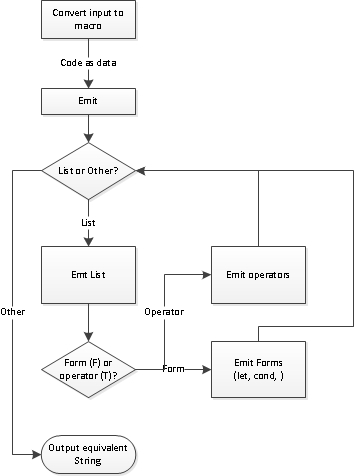
\includegraphics{Graphics/implementation_flowchart.jpg}
	\caption[yadayada]
   {Flow chart of \textit{Lispish to JavaScript} compilation.}
\end{figure}

Figure ~\ref{fig:recursive_expansion_flowchart} illustrates the functional flow chart of the compiler, without yet going deep into the details how s-expressions with multiply arity arguments are handled. 

\subsection{Forms with multiple arity (Map and reduce fns?)}

In order to solve the multiple arity problem, where for instance a (cond ) form can take multiple condition/true-form expression tuples and each one of them has to be individually compiled and them reduced to a string, a Map Reduce construct has been used. 

\subsubsection{Map}
The idea behind the map operation is to apply a function that takes one argument, to all of the elements in a collection and return a new collection with results of each application of the aforementioned function. 
A simple example of Map is 

\begin{verbatim}
(map (fn [x] (+ x 1)) 
	 [0 1 2 3 4 5])
\end{verbatim}
that yields 
\begin{verbatim}
[1 2 3 4 5 6]
\end{verbatim}
as a result

\subsection{Reduce}
Reduce generates a single result or a collection out of the application of a funcion to a collection.	

\begin{verbatim}
(reduce str 
	 [1 2 3])
\end{verbatim}
that yields 
\begin{verbatim}
"123"
\end{verbatim}
as a result. The collection of numbers has been reduced to a string, as each number was converted to a string and then a string of the collection has been produced.
If we would to map a "str" function over the collection of [1 2 3], it would result in a new collection containing all of the elements of the old collection converted to a string, namely this list ("1" "2" "3").

To now put the map reduce constructs into perspective with Lispish, here is how a multiple arity cond (allowing practically not bound list of tests) is implemented, that not only allows for multiple arity but also generates a different, yet equivalent JavaScript code: 

\begin{verbatim}
(defn emit-cond [head [name condition statement & rest]]
  (str "if(" (emit condition) ") { return " (emit statement) " }"
       (reduce str (interleave (map #(str "else if(" % ")")
                                    ;; Special case if condition is :else then emit "true"
                                    (reduce list (map #(if (= (str %) ":else") "true" (emit %))
                                                     (take-nth 2 rest))))
                               (map #(str "{ return " % " }")
                                    (map emit (take-nth 2 (pop rest)))))) ))
\end{verbatim}

Given an arbitrary number of (cond (test) result) test-result tuples, we are first emiting the first condition and the result statement. The next step is to emit and interleave the else if and return parts of the JavaScript code, with the exception of the form ":else" which needs to produce and "else if (true)" and the second part of the tuple, which is the matching true form expression.
At the end of the emiting, we are reducing the interleaved emitted JavaScript snippets to a single combined string, which results in an elegant transformation of a Lisps (cond (test) true (test2) true2) to a JavaScript if-else-if expression.

\section{Testing}
In order to test the compiler, we need ...

Let's begin our tests by a simple arithmetic expression:
\begin{verbatim}
lispish.core> (lisp-to-js (+ 2 2))
Emit Lispish:  (+ 2 2)
Emit-list head:  + , tail:  (2 2)
Emit-op, head:  + , tail:  (2 2)
Emit Lispish:  2
Emit Lispish:  2
"(2+2)"
\end{verbatim}
As we can see, our recursion begins with passing the Lispish source code to a lisp-to-js macro, which then begins the recursion by invoking the initial emit step.
At first, our s-expression is of the form (+ 2 2), which is a list. This means that the compiler has to expand the list and emit each individual expression within it. It begins by evaluating the head of the list, which happens to be an "op" operator, in this case the "+" sign. 
It therefore passes the head of the previous s-expression (the "+" sign), as well as the remaining part of the expression (2 2) to emit-op. 
Emit-op outputs the corresponding JavaScript by first mapping the top-level recursion emit function to each element inside of the tail list (2 2) which reaches the bottom of the recursion in one step each and then reduces the result of this to a string concatenated with the operator in the middle.
The same procedure is repeated for all of the "op", as well as "bop" expressions.

In the next sub section, we will have a look at a more complex example of generating a named function that is implemnted largely with Abstract Structural Binding.

\subsection{Abstract Structural Binding}
Abstract Sutrctural Binding in simple words means destructuring. It allows for destructuring any data structure to a corresponding argument in function parameters or a let form.
For example, if we define a let as follows:
\begin{verbatim}
(let [[x1 x2] [1 2]])
\end{verbatim}
"x1" will yield 1 and "x2" will yield 2.
The same principle is true for a function.
If our function accepts one parameter which is a collection:

\begin{verbatim}
(defn test [[x1 x2]] (println x1 x2))
(test [1])
\end{verbatim}
and it destructures the first two elements of the collection to x1 x2, in the above case, x1 will yield 1 and x2 null.


Lispish uses destructuring for generating all of its forms ($F$):
\begin{verbatim}
lispish.core> (lisp-to-js (defn square [x] (* x x)))
Emit Lispish:  (defn square [x] (* x x))
Emit-list head:  defn , tail:  (square [x] (* x x))
Emit-forms, head:  defn , full expression:  (defn square [x] (* x x))
Emit-defn, name:  square , arg:  x , arg tail:  nil , rest:  ((* x x))
Emit Lispish:  ((* x x))
Emit Lispish:  (* x x)
Emit-list head:  * , tail:  (x x)
Emit-op, head:  * , tail:  (x x)
Emit Lispish:  x
Emit Lispish:  x
"function square(x) {(x*x)}"
\end{verbatim}

In order to split the "defn" expression into into its respective elements, the emit-defn function that gets invoked by emit-list (after determining the head of list to be "defn") performs a structural binding of the function arguments. The bindings are then used to generate the equivalent JavaScript code. 

Lets look at the signature of the emit-defn function:
\begin{verbatim}
(defn emit-defn [type [defn name [arg & more] & rest]]
  )
\end{verbatim}
as we can see, the function takes 4 arguments and 2 optional tail arguments that can be a list of an arbitrary length. The "type" argument is simply a convinience placeholder for the head of the whole expression.
The actual expression begins to bind from the [defn name [arg \& more] \& rest] arguments. 
The optional more in the arguments list of arguments allows for an arbitrary length of the named function arguments and the optional rest is for the expression that follows the named function.

This structure can be then reused to output the corresponding JavaScript as follows:

\begin{verbatim}
(str "function "
  // Name of the function 
  name "("
    (if (nil? more) 
      // If arguments are not a list, then output just single argument
      arg 
      // Else output that list of arguments, separated by a comma
      (str arg ", " (clojure.string/join ", " more))
    )
    // Close the arguments parenthesis and begin function body
    ") {"
    // Emit function body
    (emit rest)
    // Close function body
    "}"
)
\end{verbatim}

\subsection{Automating tests with clojure.test API}
In order to ensure that the compiler is naturally expanded and all of the of regression tests are performed whenever a new language construct is added, I have decided to use the Test Driven Development methodology to approach this project. 
The tool to support me in the task of TDD I used was the clojure.test API.
clojure.test API [REFERENCE HERE] is a unit testing framework that provides a set of in-built forms, particularly the "is" macro that allows to perform boolean assertions on arbitrary expressions. 

\begin{quote}
\begin{verbatim}
(deftest factorial-example
  (is (= "function factorial(n) {if(n<2) { return 1 } else { return (n*factorial(((n-1)))) }}"
         (lisp-to-js (defn factorial [n] (if (< n 2) 1 (* n (factorial (- n 1)))))))))
\end{verbatim}
\end{quote}

.Although the compiler is not a very complexy system, it still 